\documentclass[deutsch]{lib/llncs/llncs}
\usepackage{lib/llncs/llncsdoc}
\usepackage[ngerman]{babel}
\usepackage[utf8]{inputenc}
\usepackage{hyperref}
\usepackage{graphicx}
\usepackage{lib/picins/picins}
\usepackage[nottoc]{tocbibind}


\begin{document}
\markboth
{Digitale Transformation: Schafft europäische Verordnung den Durchbruch qualifizierter elektronischer Signaturen?}
{Digitale Transformation: Schafft europäische Verordnung den Durchbruch qualifizierter elektronischer Signaturen?}
\thispagestyle{empty}


\begin{flushleft}
\LARGE\bfseries Digitale Transformation: Schafft europäische Verordnung den Durchbruch qualifizierter elektronischer Signaturen?


\end{flushleft}
\rule{\textwidth}{1pt}
\vspace{2pt}


\begin{flushright}
\Huge


\begin{tabular}{@{}l}
Interdisziplinäre und \\
sozialwissenschaftliche \\
Reflexion der Informatik 2\\\\
Wintersemester 2017/2018\\\\
Frank Dreyer\\
Matrikelnummer: 741827\\\\
07.02.2018\\[6pt]
\end{tabular}


\end{flushright}
\rule{\textwidth}{1pt}
\vfill

\newpage
\tableofcontents
\newpage\vspace{2pt}


\section{Abstract}
Genehmigungen begleiten Unternehmen weltweit beim täglichen Arbeitsalltag, sei es der Antrag auf Urlaub oder die Genehmigung eines Projekts beim Kunden. All diese Einwilligungen werden momentan noch vorrangig handschriftlich unterzeichnet, was nicht nur mit einem hohen Archivierungsaufwand verbunden ist, sondern auch die Kosten eines Unternehmens in die Höhe treiben kann. Experten schätzen, dass jede Transaktion, die Papier, Drucken, Unterschreiben, Scannen, Versand, Archivierung und Ersatz verlorengegangener Dokumente einschließt, 30 Euro für ein Unternehmen verursacht. \\
Eine Alternative zur handschriftlichen Unterschrift bilden 'qualifizierte elektronische Signaturen'. Diese Signaturverfahren arbeiten vollkommen papierfrei und sichern anhand eines asymmetrischen kryptographischen Verfahren neben der Authentizität eines Dokuments auch die Datenintegrität ab, was ein hohes Maß an Sicherheit garantiert und sie vor dem Gesetzgeber gleichermaßen anerkennen lässt, wie von Hand gefertigte Signaturen auf Papier. \\
Trotz all dieser Vorteile werden qualifizierte elektronische Signaturen im Geschäftsumfeld bisher wenig eingesetzt. Eine 2016 in Kraft getretene Signatur-Verordnung der europäischen Union verspricht Besserung: \\\\
Bisherige Akzeptanzdefizite qualifizierter elektronischer Signaturen werden durch die 'Verordnung über elektronische Identifikation und Vertrauensdienste für elektronische Transaktionen im Binnenmarkt' überwunden und zu einem breiten Einsatz der Technologie bei Geschäftsprozessen im Unternehmensbereich führen. \\\\
Diese Arbeit zeigt, warum qualifizierte elektronische Signaturen im Geschäftsumfeld bisher wenig eingesetzt wurden und warum qualifizierte Fernsignaturen, die mit der neuen europäischen Verordnung möglich werden, nun eine breite Akzeptanz bei Unternehmen finden werden. \\
Um die Akzeptanz in diesem Kontext zu evaluieren, wird das \textit{Technology Acceptance Model} angewandt.
Dafür wird zunächst der im Modell spezifizierte wahrgenommene Nutzen und wahrgenommene Bedienungskomfort dieser Technologie untersucht, um dann in einem abschließenden Fazit auf die Akzeptanz zu schließen. 


\newpage


\section{Grundlagen}


\subsection{Technology Acceptance Model}
Das \textit{Technology Acceptance Model} \cite{Zitat01}, kurz TAM, ist ein von von Fred D. Davis entwickeltes Akzeptanzmodell, welches auf dem sozialpsychologischem Modell \textit{Theory of Reasond Action} (TRA) von Ajzen und Fishbein \cite{Zitat04} basiert. Das Modell zielt darauf ab, Erkenntnisse darüber zu gewinnen, ob und warum Personen Technologien akzeptieren oder diese ablehnen. \\
Dabei wird angenommen, dass eine Person mit positiver Nutzungseinstellung zur Technologie diese auch tatsächlich verwendet. (Vgl. \cite[S. 237]{Zitat03}) Diese Nutzungseinstellung hängt wiederum maßgeblich von den Faktoren 'wahrgenommener Nutzen' und 'wahrgenommener Bedienungskomfort' ab. \\
Der 'wahrgenommene Nutzen' beschreibt das subjektiv Empfinden, dass sich eine Technologie positiv auf die Steigerung der eigenen Arbeitsleistung in einem organisatorischem Kontext auswirkt.  (Vgl. \cite[S. 320]{Zitat02}) \\
Der 'wahrgenommene Bedienungskomfort' bezeichnet das subjektive Empfinden, dass die Verwendung einer Technologie mit wenig Aufwand verbunden ist, bzw. dass die Technologie einfach zu benutzen ist. (Vgl. \cite[S. 320]{Zitat02}) \\
Bandow und Holzmüller fassen die Auswirkung dieser beiden Determinanten folgendermaßen zusammen: ''Je größer der Nutzen eines Informationssystems und je einfacher dessen Bedienbarkeit, desto eher ist der Anwender dazu bereit, das neue System zu nutzen.'' (Vgl. \cite[S. 237]{Zitat03}) \\
Auf den 'wahrgenommenen Nutzen' wie auch den 'wahrgenommenen Bedienungskomfort' wirken wiederum 'externe Variablen', die unter anderem demografische und persönliche Merkmale des Akteurs umfassen, im Originalmodell allerdings nicht weiter spezifiziert werden. (Vgl. \cite[S. 21]{Zitat01}) \\
Abbildung 1 illustriert das Modell.
\begin{figure}
	\centering
	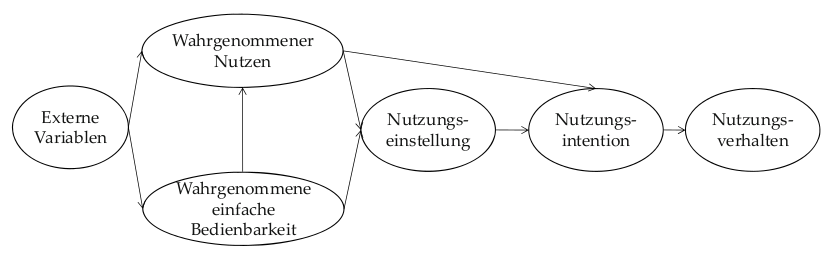
\includegraphics[scale=0.40]{img/abbildung1.png}
	\caption{\textit{Technology Acceptance Model} (Vgl. \cite[S. 237]{Zitat03})}
\end{figure}


\subsection{Digitale Signaturen}
Digitale Signaturen sind in Grenzen vergleichbar mit konventionellen Unterschriften auf Papier, welche über ein asymmetrisches kryptographisches Verfahren digitalisiert wurden. (Vgl. \cite[S. 297]{Zitat06}) Dieses asymmetrische Kryptosystem schließt drei Prozesse mit ein: den 'Unterschriftsprozess', den 'Authentifizierungsprozess' sowie den 'Prozess zur Sicherung der Datenintegrität'. (Vgl. \cite[S. 4]{Zitat05}) \\
Beim 'Unterschriftsprozess' muss sich die Person, die das jeweilige Dokument unterzeichnen soll, zunächst identifizieren. Die Identifikation hängt von der Implementierung ab und kann dementsprechend unter anderem über eine PIN, ein Passwort oder auch einen sequenz-basierten Token-Code abgewickelt werden. Ist die Identität des Unterzeichners bestätigt, so erhält er ein Zertifikat mit seiner Identität und einem öffentlichem und privatem Schlüsselpaar, mit dem er das Dokument signieren kann. Dafür wird zunächst ein einzigartiger mathematischer Code aus dem Dokument generiert, der im Anschluss über den privaten Schlüssel verschlüsselt bzw. ''signiert'', wird. Um den 'Unterschriftsprozess' abzuschließen wird das Dokument zusammen mit der Signatur (dem verschlüsseltem mathematischen Code) an den Empfänger gesandt. (Vgl. \cite[S. 4]{Zitat05}) \\
Der Empfänger kann daraufhin im 'Authentifizierungsprozess' überprüfen, ob das Dokument auch von der richtigen Person unterzeichnet wurde. Dafür fordert er den öffentlichen Schlüssel der Unterzeichners an und kann daraufhin mit dem öffentlichen Schlüssel den mathematischen Code entschlüsseln. Das Entschlüsseln wird nur dann funktionieren, wenn das Dokument mit dem korrespondierenden privaten Schlüssel verschlüsselt wurde und kann daraus folgernd auch die Authentizität garantieren. (Vgl. \cite[S. 4]{Zitat05}) \\
Zum Schluss wird im 'ProzeDie europäische Signaturgesetzgebung (eIDAS) ermöglicht das bisherige Defizit an Akzeptanz von qualifizierten elektronischen Signaturen zu überwinden.ss zur Sicherung der Datenintegrität' überprüft, ob das Dokument nach dem Signieren nicht mehr verändert wurde. Dafür wird erneut der mathematische Code aus dem Dokument generiert und mit dem im 'Authentifizierungsprozess' entschlüsselten mathematischen Code verglichen. Beide müssen identisch sein um sicher zu sein, dass das Dokument nach dem Unterschreiben nicht modifiziert wurde.  (Vgl. \cite[S. 4]{Zitat05})


\subsection{Qualifizierte elektronische Signaturen}
Von Qualifizierten Signaturen spricht man, wenn die Erzeugung einer digitalen Signatur dezentral über eine sichere Signaturerstellungseinheit abgewickelt wird und die Signatur auf qualifizierten Zertifikaten beruht. (Vgl. \cite[S. 8]{Zitat07}) \\
Die Signaturstellungseinheit, die auch Zertifizierungsstelle, Zertifizierungsdienstleister, \textit{Certification Authority} (CA) oder auch \textit{Public Key Infrastructure} (PKI) genannt wird, muss dabei vom Unterzeichner, als auch allen, die sich auf die Signatur verlassen oder berufen wollen, vertraut werden. (Vgl. \cite[S. 9]{Zitat07}) \\
Darüber hinaus sind Zertifizierungsstellen, wie der Name bereits andeutet, für die Vergabe qualifizierter Zertifikate verantwortlich. 
Diese Zertifikate müssen bestimmte Angaben, wie z.B. den Namen des Inhabers, Angaben des Signaturschlüssels und den Gültigkeitszeitraum des Zertifikats enthalten. Außerdem müssen vor der Erstellung eines Zertifikats die Identität des zukünftigen Inhabers anhand von Ausweispapieren geprüft werden und der Zertifizierungsdienstleister muss die Zertifikate über einen Zeitraum von mindestens fünf Jahren über offene Kommunikationskanäle für jedermann öffentlich zugänglich machen. (Vgl. \cite[S. 9]{Zitat07}) 


\subsection{Qualifizierte Fernsignaturen}
Von qualifizierten Fernsignaturen spricht man, wenn bei einer qualifizierten qlektronischen Signatur der private Schlüssel des Zertifikatinhabers bei der Signaturstellungseinheit liegt und von ihr verwaltet wird, wodurch der Signierer keine Smartcards, bzw. Speichermedien mit dem zugehörigen privaten Schlüssel bei sich tragen muss. (Vgl. \cite[S. 30]{Zitat08})


\section{Der wahrgenommene Nutzen qualifizierter elektronischer Signaturen}


\subsection{Effizienzsteigerung und Kostenminimierung dank schlanker Prozesse}
Geschäftsabschlüsse, die mit einer handgeschriebene Unterschrift auf Papier durchgeführt werden, haben zwei entscheidende Nachteile: Sie verzögern die Wirtschaftlichkeit und steigern die Komplexität durch Archivierung. (Vgl. \cite[S. 3]{Zitat05})\\
Diese Nachteile können mit qualifizierten elektronischen Signaturen, die über eine Zertifizierungsstelle durchgeführt und verwaltet werden, vermieden werden. Genehmigungen, die bisher durch Prozesse wie Drucken, Versand, Scannen und Archivierung viel Zeit in Anspruch und Kosten durch Papier und Personal verursacht haben, können dadurch praktisch ohne Zeitverzögerung kostengünstig abgewickelt werden und sind dank der Verwaltung durch die Signaturstellungseinheit leicht und jeder Zeit einsehbar. \\
Dieser Sachverhalt wird auch in einer von Arthur D. Little durchgeführten Befragung von 50 Marktexperten bestätigt. Sie schreiben: ''Viele Unternehmen und Behörden haben bereits das Potential dieser Technologie erkannt. Ein vollständig digitaler Prozess für die Signierung und den Versand von Dokumenten senkt die Arbeitszeiten und Kosten für Papier und Transport.'' (Vgl. \cite[S. 7]{Zitat05})
Darüber hinaus nennen die Teilnehmer der Befragung die Kosten- wie auch die Zeitersparnis als die zwei wichtigsten Vorteile beim Einsatz von digitalen Signaturen. (Vgl. Abbildung \cite[S. 7]{Zitat05})
Zwar könnte man argumentieren, dass digitale Signaturen aufgrund der Implementierung hohe Kosten verursachen. Allerdings werden diese entstandenen Kosten schnell durch reduzierte Kosten aufgewogen. (Vgl. \cite[S. 7]{Zitat05})


\subsection{Rechtsgültige Sicherheitsgarantie durch asymmetrisches Kryptosystem}
Damit eine Willenserklärung verbindlich und vor Gericht gültig ist, muss eine Authentizität bzw. Nichtabstreitbarkeit gewährleistet sein. In Schriftform wird dies durch eine eigenhändige Namensunterschrift erreicht. (Vgl \cite[S. 5-6]{Zitat07}) Diese Art der Unterschrift birgt allerdings einige Gefahren in Bezug auf die Sicherheit. So können von Hand gefertigte Unterschriften leicht von Personen gefälscht werden , die sich als Willenserklärende ausgeben. Darüber hinaus können unterschriebene Dokumente im Nachhinein von Unberechtigten modifiziert werden. Zwar werden solche Fälle der Urkundenfälschung meistens aufgeklärt, allerdings zeigt die polizeiliche Kriminalstatistik des Bundeskriminalamts aus dem Jahr 2016, dass es mit einem verhältnismäßig hohen Anteil von 16,4 \% immer noch Urkundenfälschungsdelikte gibt, die nicht aufgeklärt werden können. (Vgl. \cite[S. 34]{Zitat10})\\
Qualifizierte Fernsignaturen verwenden eine ganz andere Taktik. Sie benutzen ein asymmetrisches kryptographisches Verfahren um die Authentizität zu gewährleisten. Dafür muss sich die für die Unterschrift berechtigte Person zunächst mittels einer 2-Faktor-Authentifizierung bei der Signaturstellungseinheit identifizieren, die bei Erfolg den Prozess des Signierens für den identifizierten Zertifikatinhaber einleitet. Damit die Signaturstellungseinheit als ''qualifizierter Vertrauensdienst'' (Vgl. \cite[S. 30]{Zitat08}) operieren darf, müssen gemäß der EU-Verordnung eIDAS gewisse Sicherheitskriterien erfüllt sein: So müssen ''Anbieter von elektronischen Fernsignaturdiensten spezielle Verfahren für die Handhabung und Sicherheitsverwahrung mit vertrauenswürdigen Systemen und Produkten anwenden, u. a. durch abgesicherte elektronische Kommunikationskanäle, um für eine vertrauenswürdige Umgebung zur Erstellung elektronischer Signaturen zu sorgen und zu gewährleisten, dass diese Umgebung unter alleiniger Kontrolle des Unterzeichners genutzt worden ist.'' (Vgl. \cite[S. 233]{Zitat09}) Des Weiteren muss sich der qualifizierte Vertrauensdienst einer Konformitätsprüfung unterziehen, die alle 24 Monate wiederholt wird und überprüft, ob alle in der eIDAS-Verordnung festgelegten Anforderungen erfüllt sind. (Vgl. \cite[S. 30]{Zitat08}) \\
Ein weiterer wichtiger Mehrwert von digitalen Signaturen, der bei herkömmlichen eigenhändigen Namensunterschriften fehlt, ist die Integritätsprüfung, die die Manipulation eines Dokuments praktisch unmöglich macht. (Vgl. \cite[S. 7]{Zitat05}) \\
Eine Kombination der beiden Sicherheitsfaktoren Authentizität und Integrität ist gerade bei Geschäftstransaktionen entscheidend, da in diesem Umfeld mit sensitiven und vertraulichen Daten gearbeitet wird. (Vgl. \cite[S. 7]{Zitat05})


\subsection{Weitere Besonderheiten digitalisierter Willenserklärungen}
Neben der effizienzsteigernden, kostenminimierenden und sicherheitsgarantierenden Eigenschaften, die qualifizierte elektronische Signaturen mit sich bringen, haben sie eine Reihe weiterer Besonderheiten, die vor allem bei Transaktionen im Geschäftsumfeld den Unterschied machen. \\
Unternehmen die sich bei ihren Geschäftspartnern und Kunden fortschrittlich repräsentieren wollen, haben mit digitalen Signaturen ein hervorragendes Werkzeug dafür. Sie vertreten damit ein innovatives Image sowohl für Nutzer als auch für Anbieter der Technologie, was sich im Rückschluss auf eine positive Kundenzufriedenheit auswirkt. (Vgl. \cite[S. 7]{Zitat05}) Dieses Image spiegelt sich auch bei Transaktionen zwischen Unternehmen wieder, wo ''technologisch fortgeschrittene Geschäftspartner als Rollenmodelle dienen.'' (Vgl. \cite[S. 12]{Zitat05}) \\
Ein weiterer Vorteil ist der Zeitstempel, welcher zu einer digitalen Signatur hinzugefügt werden kann. So ist es möglich sicher zu stellen, dass ein Dokument zu einem bestimmten Datum signiert wurde. (Vg. \cite[S. 7]{Zitat05}) Ist ein Dokument zu einem bestimmten Termin zu unterschreiben, z.B. bei einer Kündigung, kann dieser exakt bestimmte Zeitstempel der Unterschrift helfen Betrug auszuschließen. \\
Die eIDAS-Verordnung, welche 2016 in Kraft getreten ist, macht es des weiteren möglich sogenannte 'elektronische Siegel' oder 'E-Siegel' einzusetzen. Jene sind qualifizierte Signaturen, die nicht einer Person sondern einer Organisation zugeordnet werden, was insbesondere für Unternehmen interessant werden könnte. Geschäftseinwilligungen, die einen Firmenstempel erfordern, können dementsprechend auch digitalisiert werden und folglich Prozesskosten minimieren. (Vgl. \cite[S. 30-31]{Zitat05})


\subsection{Zwischenfazit: Wird der Nutzen von qualifizierten elektronischen Signaturen wahrgenommen?}
Diese Frage ist mit einem eindeutigen Ja zu beantworten. Qualifizierte elektronische Signaturen lassen Unternehmen schneller bei Geschäftsabschlüssen agieren, sind sicherer und kostengünstiger als herkömmliche von Hand gefertigte Namensunterschriften und bieten weitere nützliche Features. \\
Firmen haben durch den Einsatz besagter Technologie das Potential nachhaltige Wettbewerbsvorteile zu erzielen, wie eine Untersuchung von Arthur D. Little und weitere Analysen bestätigen. (Vgl. \cite[S. 7]{Zitat05})
Dieses Potential wurde bereits von zahlreichen Firmen erkannt. So auch bei der \textit{Credit AgricoleConsumer Finance}, einem Anbieter von Konsumentenkrediten in Frankreich und Europa, der durch den Einsatz die Kundenzufriedenheit als innovativer Anbieter erhöhen sowie Kosten sparen konnte. \cite[S. 13]{Zitat05} \\
Zusammenfassend kann festgestellt werden, dass sich qualifizierte elektronische Signaturen positiv auf die Steigerung der eigenen Arbeitsleistung auswirkt, da nachhaltige Wettbewerbsvorteile erzielt werden können. Der wahrgenommene Nutzen ist demzufolge sehr hoch. 


\section{Der wahrgenommene Bedienungskomfort qualifizierter elektronischer Signaturen}


\subsection{Bedienungsproblematik beim bisherigen Einsatz von qualifizierten elektronischen Signaturen}
Auch wenn sich der Einsatz qualifizierter elektronischer Signaturen - dank ihrer Eigenschaften - positiv auf die Steigerung der eigenen Arbeitsleistung auswirkt, gab es bisher einige Defizite in Bezug auf die Bedienung. \\
Dieser Mangel an Bedienungskomfort ist vor allem den unterschiedlich ausfallenden Signaturgesetzgebungen der einzelnen Länder innerhalb der EU geschuldet. Zwar gab es bereits eine EU-Richtlinie, die versuchte Einigkeit digitalisierter Willenserklärungen zu schaffen, allerdings präferierten die EU-Mitglieder unterschiedliche Aspekte digitaler Signaturen, wodurch keine Einigung erzielt werden konnte. (Vgl. \cite[S. 30]{Zitat08}) Jene ''babylonische Gesetzesverwirrung'' (Vgl. \cite[S. 30]{Zitat08}) hatte zur Folge, dass die Mitglieder aufgrund variierender Sicherheitsmaßstäbe unterschiedliche Technologien für den Einsatz digitalisierter Signaturen wählten, wodurch Interoperabilität zwischen den Mitgliedern praktisch unmöglich wurde. \\
Deutschland stellte hohe Sicherheitsanforderungen an die Technologie. Qualifizierte elektronische Signaturen waren demzufolge nur gestattet, wenn ''der Signierer eine Smartcard (oder ein anderes Speichermedium) mit dem privaten Signaturschlüssel bei sich trug und unter seiner direkten Kontrolle hatte.'' (Vgl. \cite[S. 30]{Zitat08}) Qualifizierte Fernsignaturen, bei denen der private Signaturschlüssel bei der Signaturstellungseinheit erstellt und verwaltet wird, waren daher nicht erlaubt. \\
Der Einsatz solcher Smartcards bzw. Tokens erweist sich als äußerst unpraktisch in der Bedienung: So müssen zusätzliche Geräte angeschafft und Software installiert werden, um die Technologie einsetzen zu können, die dann auch noch umständlich zu bedienen sind. Diese Hürde für den Endanwender wird auch von Diplom-Betriebswirt Enrico Entschew bestätigt, der als Senior Developer für die Bundesdruckerei tätig ist: ''Je komplexer die Einsatzumgebung gestaltet ist, desto höher ist die Barriere für den Nutzer.'' (Vgl. \cite[S. 232]{Zitat09}) \\
Ein weiteres wichtiges Problem ergibt sich dadurch, dass Nutzer der Technologie gezwungen sind, die für die Signatur notwendigen Geräte immer bei sich zu tragen. Dass das den Bedienkomfort einschränkt und bei Unternehmen schlecht ankommt, spiegelt sich auch in einem Interview wieder, das Arthur D. Little durchgeführt hat. So sagt ein Studienteilnehmer: ''Warum sollten wir von unseren Kunden verlangen, ständig einen Token oder Smart-Card-Reader bei sich zu tragen?'' (Vgl. \cite[S. 5]{Zitat05}) \\
All diese Komfortdefizite in der Bedienung haben letztendlich dazu geführt, dass qualifizierte elektronische Signaturen bisher eher als technische Spielerei anstelle einer ernsthaften Innovation angesehen wurden.  (Vgl. \cite[S. 29]{Zitat08})


\subsection{Besserung durch eIDAS}
eIDAS hat das Ziel diese Problematik zu lösen. So sollen zwei Aufgaben gleichzeitig erfüllt werden: Digitale Signaturen sollen zum Einen einfacher werden, ohne die Sicherheit zu beeinträchtigen und zum Anderen EU-weit harmonisiert werden. (Vgl. \cite[S. 33]{Zitat08}) Diese Ziele werden durch juristische und technische Rahmenbedingungen erreicht, die eIDAS vorgibt. \\
Was die juristischen Rahmenbedingungen betrifft, ermöglicht eIDAS eine Vereinheitlichung der Rechtslage in der EU und die gegenseitige Anerkennung von digitalen Signaturen. (Vgl. \cite[S. 33]{Zitat08}) \\
Für die technischen Rahmenbedingung, werden die bisher meist als umständlich zu bedienenden Lösungen für qualifizierte elektronische Signaturen durch die Möglichkeit der Fernsignatur vereinfacht (Vgl. \cite[S. 30]{Zitat08}), die in jedem EU-Mitgliedstaat gleichermaßen anerkannt wird. \\
Jene qualifizierte Fernsignaturen ermöglichen dem Anwender nur noch die für die Signaturerzeugung erforderlichen Authentifizierungsmittel in seiner alleinigen Kontrolle zu halten, ohne ein Gerät mit dem privaten Signaturschlüssel ständig bei sich tragen zu müssen, was ein hohes Maß an Benutzerfreundlichkeit bietet. So können Anwender ohne eine umfangreiche Änderung der gewohnten Einsatzumgebung, plattformunabhängige qualifizierte elektronische Signaturen mit nichts anderem als einem gewöhnlichen Internetbrowser erzeugen.  Sollte es nötig sein Schlüsselmaterial und das zugehörige qualifizierte Zertifikat für einen bereits identifizierten Nutzer zu erneuern, wird dies beim Zertifizierungsdienstleister unmittelbar zentral abgewickelt, ohne dass der Anwender davon etwas mitbekommt. (Vgl. \cite[S. 233-234]{Zitat09})\\
Um den notwendigen Sicherheitsansprüchen einiger EU-Mitgliedstaaten gerecht zu werden, müssen Signaturstellungseinheiten, die diese Technologie der Fernsignatur anbieten, bestimmte Sicherheitskriterien erfüllen, die unter anderem eine 2-Faktor-Authentifizierung mit einschließt. \\
Es gibt mittlerweile Zahlreiche Verfahren für die 2-Faktor-Authentifizierung, die ein hohes Maß an Bedienkomfort erfüllen. \\
Der offene und lizenzfreie Standard \textit{Unsiversal Second Factor} (U2F), welches von der \textit{Fast Identity Online}-Allianz (FIDO-Allianz) entwickelt wurde, ist ein solches Verfahren, welches bereits breite Unterstützung von Google und Microsoft erfährt. Es ermöglicht eine nicht nur einfache sondern auch sichere 2-Faktor-Authentifizierung über ein klassisches Challenge-Response-Protokoll mittels eines FIDO-Tokens. Eine Installation von Soft- oder Hardwarekomponenten ist dabei nicht erforderlich, da alles bereits im verwendeten  Browser bzw. Betriebssystem bereitgestellt wird. (Vgl. \cite[S. 234]{Zitat09}) \\
Des Weiteren wird an einer 2-Faktor-Authentifizierung gearbeitet, die vollkommen ohne Token arbeitet. Dabei soll die Authentifizierung über ein Passwort und eine mobile Transaktionsnummer, die an das Smartphone des Anwenders gesendet wird, erfolgen. Damit es sich auch hier um eine gültige 2-Faktor-Authentifizierung handelt darf das Gerät, welches die Signatur anstößt nicht das selbe sein, was die TAN erhält. An dieser Problematik wird derzeit gearbeitet. (Vgl. \cite[S. 32]{Zitat08})


\subsection{Zwischenfazit: Wird der Bedienungskomfort von qualifizierten elektronischen Signaturen wahrgenommen?}
Auch diese Frage ist, dank der neu geltenden eIDAS-Verordnung und ihrer technischen und juristischen Neuerungen, mit einem Ja zu beantworten. Wo die Bedienbarkeit von qualifizierten elektronischen Signaturen bisher wenig Akzeptanz gefunden hat, aufgrund der Installation und komplizierten Nutzung notwendiger Hard- und Software sowie der nicht gegebenen Interoperabilität und gleichmäßigen Anerkennung zwischen den EU-Ländern, schaffen qualifizierte Fernsignaturen eine einfache und trotzdem sichere Alternative, die alle EU-Mitglieder mit ihren Geschäftsprozessen untereinander näher zusammenbringt. \\
Alles in allem lösen die eIDAS-Verordnung und die daraus resultierenden qualifizierten Fernsignaturen die Bedienungsprobleme, welche Anwender mit der bisherigen Umsetzung qualifizierter elektronischer Signaturen hatten, weswegen der wahrgenommene Bedienungskomfort als hoch erachtet werden kann.


\section{Fazit}
Qualifizierte elektronische Signaturen haben aufgrund ihrer effizienzsteigernden, kostenminimierenden und sicherheitsgarantierenden Eigenschaften, die von Hand gefertigte Unterschriften auf Papier bei weitem übertreffen, einen hohen Nutzfaktor für Unternehmen. \\
Trotz allem wurden Lösungen genannter Technologie im Unternehmenskontext bisher wenig eingesetzt. Das liegt daran, dass die Bedienung solcher Lösungen zu aufwendig und komplex ist und eine Interoperabilität zwischen den EU-Mitgliedern nicht zulässt, weswegen der Bedienungskomfort für den Anwender eingeschränkt ist. Da neben dem wahrgenommenen Nutzen auch der wahrgenommene Bedienungskomfort eine essentielle Rolle im \textit{Technology Acceptance Model} spielt, kann auf die Nichtakzeptanz besagter Lösung im Unternehmenskontext geschlossen werden. \\
Die eIDAS-Verordnung hat grundlegendes verändert. Sie schafft Klarheit, was die gleichmäßige Anerkennung zwischen EU-Mitgliedern bezüglich qualifizierter elektronischer Signaturen betrifft und vereinfacht die Bedienbarkeit der Technologie durch eine komfortable Lösung der qualifizierten Fernsignatur, die trotz ihres Komforts sicher ist. Bisherige Problematiken in der Bedienung werden folglich durch die eIDAS-Verordnung gelöst und resultieren in einem hohen wahrgenommenen Bedienungskomfort. \\
Gemäß des \textit{Technology Acceptance Model} stellen ein hoher wahrgenommener Nutzen sowie Bedienungskomfort die beste Voraussetzung für die Akzeptanz und der damit verbundene Einsatz der Technologie. \\
Zusammengefasst kann gesagt werden, dass qualifizierte elektronische Signaturen mit der Lösung einer Fernsignatur, breite Akzeptanz in Unternehmen finden und diese in Zukunft häufiger für geschäftliche Willenserklärungen zum Einsatz kommen werden.


\bibliographystyle{amsalpha}
\bibliography{lit/lit}


\end{document}
